\chapter{The ML correction: what went wrong and how we fixed it}
\label{ch:mlstory}

This part is the longest on purpose. If the evaluator asks only one hard question, it will be about the ML, and the best answer is the true story told in order.

\section{The timeline}
\begin{enumerate}
\item \textbf{Version 1.} A per-service Isolation Forest, a random walk to rank causes, a hybrid with the rules. It scored well on our injected-fault benchmarks.
\item \textbf{The report.} Stopping the traffic generator and switching to ML made \emph{every service show a 100\% anomaly score}. Nothing was broken.
\item \textbf{Reproducing it.} We recorded fault-free runs where only the workload changed. In the first set the organic traffic generator ran, stopped, ran, stopped for longer, and ran again (62 minutes). In the second, a closed-loop generator held a constant number of visitors and stepped it $2\to8\to2\to0\to20\to2$ (72 minutes). Every alarm in those recordings is a false alarm by construction.
\item \textbf{The benchmark had hidden it.} Our replay tool skipped a reading whenever it was identical to the previous one. An idle service reports the same zeros again and again, so the replay deleted the idle stretches, and the old forest looked well behaved when traffic stopped. We fixed the replay.
\item \textbf{Comparing alternatives.} We built the contenders (below) and measured them on injected faults \emph{and} on those fault-free recordings.
\item \textbf{The choice.} The load-aware residual model with a tail-aware spread.
\item \textbf{Adopting and re-running everything.} Made the default, re-ran every experiment, tests, figures and the report.
\end{enumerate}

\begin{saybox}
Tell it in this order. The shape is: \emph{we found a real failure, we reproduced it, we found out why our own benchmark had hidden it, we compared fixes fairly, we picked the one that worked, we re-ran everything.} That is a strong research story.
\end{saybox}

\section{Why the old engine failed, in one picture}
\begin{simplebox}
The forest learned the \emph{shape} of each service's recent numbers. When the traffic changed, the numbers moved to a place the forest had never seen, for all services at once. A forest cannot say ``this is just louder than before''; it only knows ``this is unlike what I have seen''. Add a safety guard that fires when a value falls outside the range seen so far, and a total traffic change makes every guard fire at the same time. On top of that, a big shift was only accepted as the new normal after thirty minutes.
\end{simplebox}

\begin{techbox}
On fault-free workload recordings the old forest was in alarm 23\% (organic on/off) and 52\% (stepped load) of the time, and raised 27.7 and 21.3 false-alarm episodes per hour. Every other workload-blind detector did the same or worse: the ensemble of four 47\% and 88\%, k-NN 73\% and 96\%, Mahalanobis 38\% and 76\%, HBOS 75\% and 82\%. Because all of them model the readings themselves, a new workload is outside what they were fitted on. A forest also scores a value beyond its training range no higher than its most extreme training point, so the engine had added a range guard, which fires at once for every service when traffic changes for all of them. On the fault-free stretches of the live fault campaigns the same engine raised 40.9 alarm episodes per hour.
\end{techbox}

\section{The contenders}
\begin{simplebox}
We tried several ways of fixing it, so nobody could say we just picked the first thing. Three families:

\begin{enumerate}
\item \textbf{More of the same.} Other ``learn the shape'' detectors (k-NN, Mahalanobis, HBOS, an ensemble). They fail the same way.
\item \textbf{Simple control chart.} Judge each number against its own history with robust statistics, no learned shape. This already helps a lot, because it does not claim to know the shape of traffic.
\item \textbf{Ones that treat the shared workload explicitly.} A subspace model (the classic multivariate monitoring idea: the shared cause is one or two ``directions'' in the data, and an anomaly is what falls off those directions), and our load-factor model.
\end{enumerate}
\end{simplebox}

\begin{techbox}
All unsupervised, all computed from telemetry the mapper already collects. (a) Forest family: Isolation Forest, ensemble, k-NN, Mahalanobis, HBOS. (b) Control chart with MAD spread or tail spread. (c) Subspace residual (principal-component residual of the standardised readings of all services, 1 or 2 components). (d) Load factor with MAD or tail spread. We also tried and rejected a range guard on the residual (it added false alarms and changed no injected-fault result) and varied the alarm line, window, slow reference and drift time.
\end{techbox}

\section{The results table, and how to read it}
\begin{figure}[H]
\centering
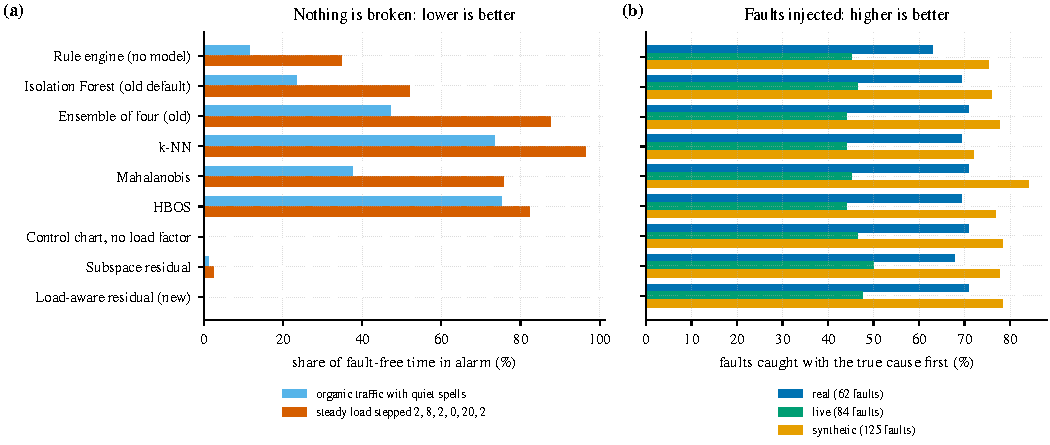
\includegraphics[width=0.98\textwidth]{fig_models.pdf}
\caption{The candidate models. (a) Share of fault-free time in alarm on the two workload recordings (lower is better). (b) Share of injected faults caught with the true cause first (higher is better).}
\end{figure}

\begin{center}
\scriptsize
\setlength{\tabcolsep}{3pt}
\begin{tabular}{lrrrrrrrr}
\toprule
 & \multicolumn{2}{c}{Real (62)} & \multicolumn{2}{c}{Live (84)} & \multicolumn{2}{c}{Synthetic (125)} & \multicolumn{2}{c}{No faults}\\
Model & C+N & FA/h & C+N & FA/h & C+N & FA/h & organic & steps\\
\midrule
Rule engine (z-score) & 63 & 9.2 & 45 & 16.3 & 75 & 2.6 & 12 & 35\\
Isolation Forest (old) & 69 & 4.6 & 46 & 40.9 & 76 & 0.2 & 23 & 52\\
Ensemble of four & 71 & 20.0 & 44 & 81.7 & 78 & 2.6 & 47 & 88\\
k-NN & 69 & 13.8 & 44 & 57.2 & 72 & 5.2 & 73 & 96\\
Mahalanobis & 71 & 23.8 & 45 & 65.4 & 84 & 2.6 & 38 & 76\\
HBOS & 69 & 34.6 & 44 & 57.2 & 77 & 1.4 & 75 & 82\\
Control chart, MAD spread & 73 & 10.0 & 44 & 24.5 & 79 & 0.6 & 13 & 31\\
Control chart, tail spread & 71 & 2.3 & 46 & 0.0 & 78 & 0.2 & 0 & 0\\
Subspace residual, 1 comp. & 68 & 3.1 & 50 & 8.2 & 78 & 0.4 & 1 & 3\\
Subspace residual, 2 comp. & 68 & 3.8 & 50 & 0.0 & 77 & 0.2 & 1 & 4\\
Load factor, MAD spread & 71 & 3.8 & 43 & 16.3 & 79 & 0.6 & 10 & 6\\
\textbf{Load factor, tail spread} & 71 & 2.3 & 48 & 0.0 & 78 & 0.2 & 0 & 0\\
\bottomrule
\end{tabular}
\end{center}

\begin{simplebox}
How to read this table in thirty seconds. \textbf{C+N} is ``caught and named'': the fault was detected \emph{and} the correct service was ranked first, in percent (higher is better). \textbf{FA/h} is false alarms per hour of fault-free time (lower is better). The last two columns are the share of time spent in alarm on recordings where \emph{nothing was broken}; every minute in alarm there is a mistake (lower is better, zero is perfect).

Look at the last two columns first: the forest family is at 23--96\%, the adopted model at 0\%. Then look at the C+N columns: they are all close, 68--84\% on the real and synthetic sets, 43--50\% on the live sets. So \emph{the models are alike at catching faults; they are not alike at staying quiet when only the workload moves.}
\end{simplebox}

\begin{techbox}
Three results stand out. (1) On injected faults the models are alike (68--73\% real, 43--50\% live, 72--84\% synthetic); differences of a few points are inside the noise of 62--125 faults. The forest-family detectors raise 4.6--34.6 episodes/h on the real systems and 40.9--81.7 on the live ones, against 2.3 and 0.0 for the adopted model. (2) On workload shifts they differ: adopted 0\% and 0\%, workload-blind family 23--75\% and 52--96\%. Replacing the forests by a robust residual with the tail-aware spread is the larger part of the improvement (control chart: 0\% and 0\%); the MAD spread alone is not enough (13\% and 31\%) because it treats bursty signals as Gaussian. (3) The load factor removes what is left: the control chart still raises 1.2 and 1.9 false episodes/h on the two recordings; with the load factor 0.0 and 1.0, and it is slightly better on the live faults (47.6\% against 46.4\% caught and named). The subspace residual is the strongest alternative (3\% and 4\% of the steady recording in alarm; 50\% C+N on live faults) but raises 7.7--10.7 false episodes/h on the steady steps, adapts more slowly and its cost grows faster than linearly.
\end{techbox}

\begin{warnbox}
Be honest about what the new model is \emph{not}: it is not more accurate than the forest at catching injected faults (71\% against 69\% on the real faults, inside the noise). The benefit is robustness: it does not mistake a workload change for a fault. Also admit that a fault that begins during a very large change of load can be masked, because both load hypotheses may explain it.
\end{warnbox}

\section{How we set its dials, and what each does}
\begin{center}
\small
\begin{tabularx}{\textwidth}{>{\raggedright\arraybackslash}p{4cm}>{\raggedright\arraybackslash}p{2.4cm}>{\raggedright\arraybackslash}X}
\toprule
\textbf{Dial} & \textbf{Value} & \textbf{What it does, in plain words}\\
\midrule
Alarm line $z_{\text{line}}$ & 4 robust spreads & How far from normal counts as ``level 1''. Looser (2) catches more faults but alarms on workloads; tighter (6--8) is silent but loses detection. 4 is the loosest value that keeps the workload recordings quiet.\\
Training window & 120 readings & About ten minutes of normal behaviour to learn from. 60 is too short (noisy again).\\
Slow reference & 360 readings & The half-hour median that shifts are measured from.\\
Readings before judging & 30 & Warm-up per service.\\
Mild drift & 24 readings & A small steady change becomes normal after 2 minutes.\\
Large drift & 360 readings & A large change needs 30 minutes.\\
Alarm level & 2 & The hybrid needs twice the line.\\
Persistence & 2 windows & The alarm must hold on two cycles in a row.\\
\bottomrule
\end{tabularx}
\end{center}

\begin{figure}[H]
\centering
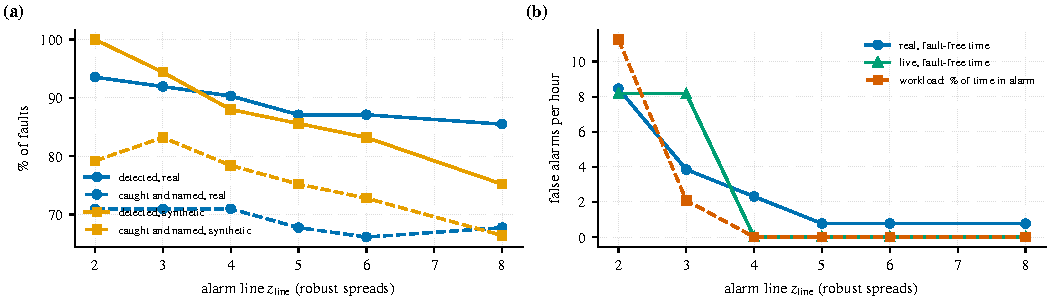
\includegraphics[width=0.98\textwidth]{fig_zline.pdf}
\caption{Sensitivity of the load-aware model to its alarm line.}
\end{figure}

\begin{warnbox}
We swept these dials on all recordings together. That is tuning on the test data, and the report says so. We chose the flat region of the sweep, not its maximum. If asked ``did you overfit the settings?'', say: ``Partly possible. The synthetic results come from a split we tuned on separately and scored once; the real-system numbers have no held-out system, so they are optimistic by an amount we cannot measure.''
\end{warnbox}

\section{The three-way comparison document}
We also wrote a standalone comparison in the repository (\code{wiki/44-ml-comparison.md}) that puts Rules, the old ML and the new ML side by side with plain-language reasons. Section 6.1.3 and Table 6.2 of the report show the same thing. The headline from it:

\begin{center}
\small
\begin{tabular}{lccc}
\toprule
 & Rules & Old ML & New ML\\
\midrule
Real faults: C+N / FA per h & 63\% / 9.2 & 69\% / 4.6 & \textbf{71\% / 2.3}\\
Live faults: C+N / FA per h & 45\% / 16.3 & 46\% / 40.9 & \textbf{48\% / 0.0}\\
Synthetic: C+N / FA per h & 75\% / 2.6 & 76\% / 0.2 & \textbf{78\% / 0.2}\\
Time in alarm, traffic on/off & 12\% & 23\% & \textbf{0\%}\\
Time in alarm, stepped load & 35\% & 52\% & \textbf{0\%}\\
Cost, 320 services (ms) & -- & 296 & \textbf{119}\\
\bottomrule
\end{tabular}
\end{center}

\begin{techbox}
Per-reading ranking (ROC): the plain rule $z$-score has the best AUROC on both sets (0.695 real, 0.873 synthetic) against 0.629 and 0.862 for the old forest and 0.665 and 0.842 for the load-aware model; the load-aware model has a higher average precision than the forest on the held-out set (0.665 against 0.528). This is not a contradiction: one high reading is cheap. What the user sees is an alarm (two cycles in a row) and a named source, and there the rules fall behind because they fire on traffic swings and blame the loudest service.
\end{techbox}

\begin{saybox}
``Honestly, per single reading the plain rule score is the best classifier. We say that in the report. The new model is not adopted because it ranks single readings better. It is adopted because it stays quiet when only the workload moves, which is the failure that an operator actually hit.''
\end{saybox}
